%\documentclass[journal]{IEEEtran}
\documentclass{article}

\usepackage{amsmath,amssymb,caption,comment,enumitem,float,graphicx,microtype}
\usepackage[utf8]{inputenc}
\usepackage[T1]{fontenc}
\usepackage[margin=1in]{geometry}
\usepackage{setspace}
\usepackage{fancyhdr}
\usepackage{bm}
\usepackage{caption}
\usepackage{subcaption}
\pagestyle{fancy}
\fancyhf{}
\rhead{\today}

\newcommand{\N}{{\mathbb N}}
\newcommand{\Z}{{\mathbb Z}}
\newcommand{\Q}{{\mathbb Q}}
\newcommand{\R}{{\mathbb R}}
\newcommand{\C}{{\mathbb C}}
\newcommand{\F}{{\mathbb F}}
\newcommand{\E}{{\mathbb E}}
\mathchardef\hyphen="2D

\title{6.867 Homework 1}
\author{Anonymous Authors}

\begin{document}

\maketitle
\thispagestyle{fancy}

\section{Implementing Gradient Descent}


In any gradient descent algorithm, the main hyperparameters we have to tune are the initial point we start the gradient descent from, the step size, and the convergence criteria. 

\begin{itemize}

\item An incorrect initial guess could lead to getting stuck at a local min without ever reaching the global minumum
\item A step size that is too large can shoot past the minumum or go back and forth without ever reaching the critical point. Conversely, a step size that is too small can make the algorithm take far too long to converge.
\item A convergence criteria that is too lax can result in a sub-optimal stopping point, while a convergence criteria that is too strict can result in the algorithm taking too long.

\end{itemize}

For each of the three parameters, we can see how varying the parameters changes the gradient descent for both of the provided functions (the Gaussian and the bowl).

Default parameters are: 

\begin{itemize}

\item Starting Point: (0,0)
\item Step Size: 0.01
\item Convergence Criteria: Difference between consecutive objective function values is less than $10^{-10}$, max of 20,000 iterations
\end{itemize}

\begin{figure}[H]
        \begin{subfigure}[b]{0.5\textwidth}
                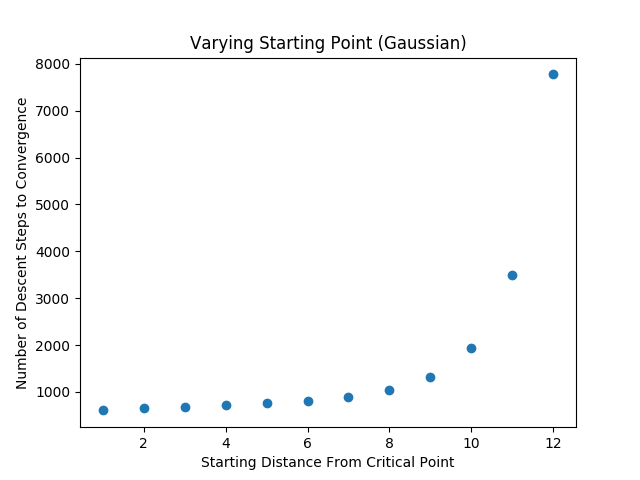
\includegraphics[width=\linewidth]{../P1/figs/start_gauss.png}
        \end{subfigure}%
        \begin{subfigure}[b]{0.5\textwidth}
                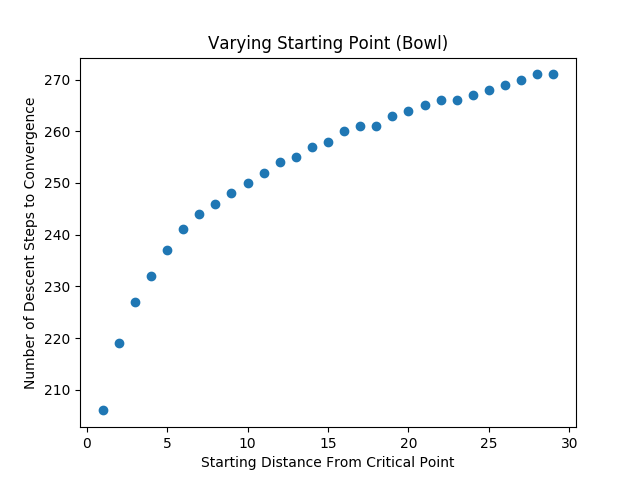
\includegraphics[width=\linewidth]{../P1/figs/start_bowl.png}
        \end{subfigure}%
	\caption*{The number of steps needed for convergence grows much faster in the Gaussian than it does with the bowl. This is because the gradient decays exponentially in the Gaussian case with respect to distance from the critical point but linearly in the bowl case.}
\end{figure}

\begin{figure}[H]
        \begin{subfigure}[b]{0.5\textwidth}
                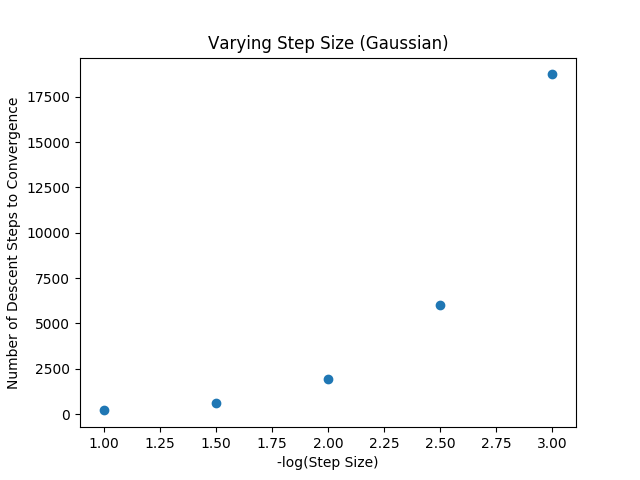
\includegraphics[width=\linewidth]{../P1/figs/step_gauss.png}
        \end{subfigure}%
        \begin{subfigure}[b]{0.5\textwidth}
                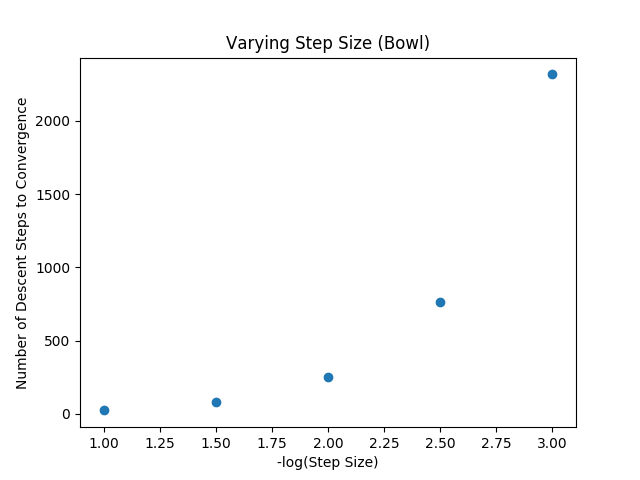
\includegraphics[width=\linewidth]{../P1/figs/step_bowl.png}
        \end{subfigure}%
\caption*{In both cases, step size eventually grows linearly with the number of steps needed until convergence. However, in some cases where the step size is extremely large (not shown), the function may not converge at all.}
\end{figure}

\begin{figure}[H]
        \begin{subfigure}[b]{0.5\textwidth}
                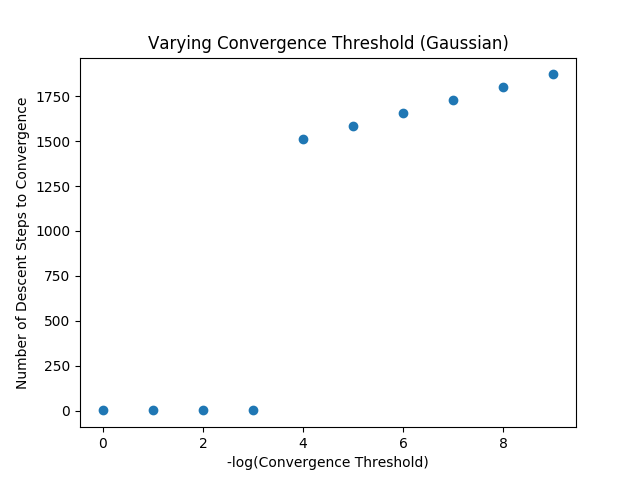
\includegraphics[width=\linewidth]{../P1/figs/converge_gauss.png}
        \end{subfigure}%
        \begin{subfigure}[b]{0.5\textwidth}
                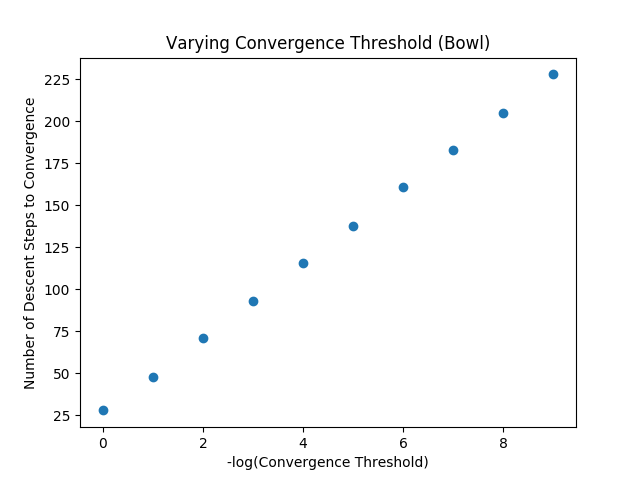
\includegraphics[width=\linewidth]{../P1/figs/converge_bowl.png}
        \end{subfigure}%
\caption*{Here, as the convergence threshold grows, so to does the number of steps needed to converge.}
\end{figure}

\begin{figure}[H]
        \begin{subfigure}[b]{0.5\textwidth}
                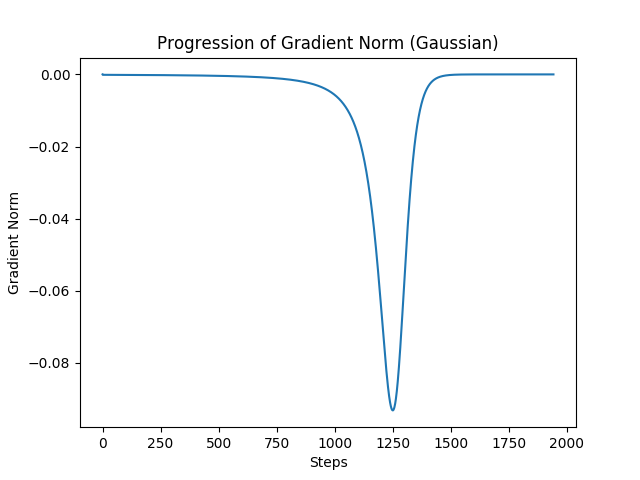
\includegraphics[width=\linewidth]{../P1/figs/grad_norm_gauss.png}
        \end{subfigure}%
        \begin{subfigure}[b]{0.5\textwidth}
                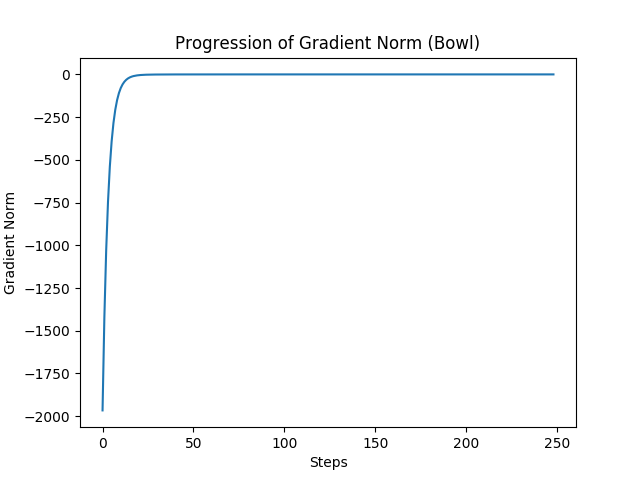
\includegraphics[width=\linewidth]{../P1/figs/grad_norm_bowl.png}
        \end{subfigure}%
\caption*{As mentioned before, the gradient norm of the Gaussian starts off very small when the starting point is far away from the critical point. Around step 1000, it starts to reach the steep part of the Gaussian, at which point it quickly reaches convergence. For the bowl, the gradient norm starts off high and quickly decreases and converges.}
\end{figure}

To perform gradient descent on functions that do not have a clean, closed-form gradient, we can approximate the gradient using central differences. Here, we analyze how the performance of the central differences approximation varies based on the step size used for the difference approximation.

\begin{figure}[H]
        \begin{subfigure}[b]{0.5\textwidth}
                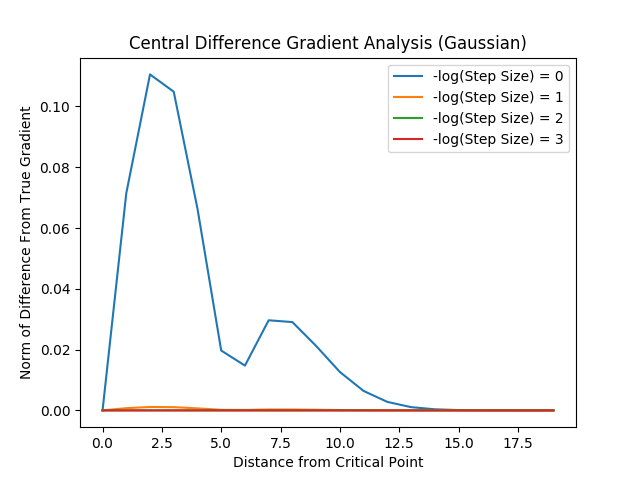
\includegraphics[width=\linewidth]{../P1/figs/central_diff_gauss.png}
        \end{subfigure}%
        \begin{subfigure}[b]{0.5\textwidth}
                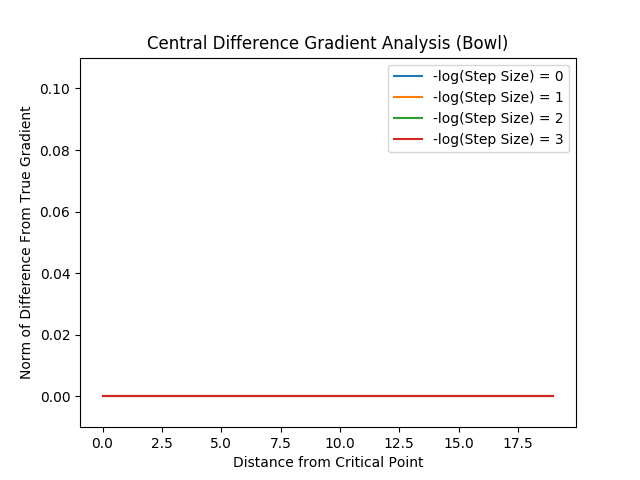
\includegraphics[width=\linewidth]{../P1/figs/central_diff_bowl.png}
        \end{subfigure}%
\caption*{When the step size is large, we see some errors in the approximate gradient norm. However, once we reach step sizes of $10^{-2}$ or smaller, the errors vanish. For the bowl, we have no error in our gradient approximation regardless of step size because the gradient of the bowl is linear. Thus, approximating the gradient of the bowl with the average of two points gives us the exact gradient.}
\end{figure}

Often, when running gradient descent, it is computationally expensive to calculate the total error. We can use Stochastic Gradient Descent as an alternative: each time we calculate the least square error, we only use one sample to calculate the error. This results in a much faster overall computation at the expense of some accuracy. We can compare the two algorithms by calculating the gradient descent of the least square error with similar convergence criteria.

\begin{figure}[H]
        \begin{subfigure}[b]{0.5\textwidth}
                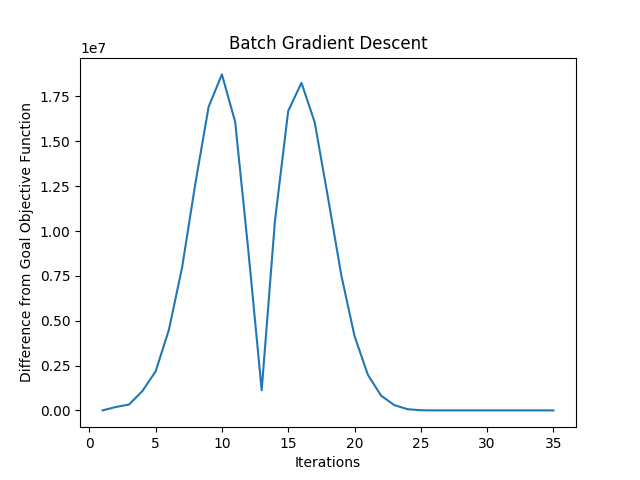
\includegraphics[width=\linewidth]{../P1/figs/plot_batch.png}
        \end{subfigure}%
        \begin{subfigure}[b]{0.5\textwidth}
                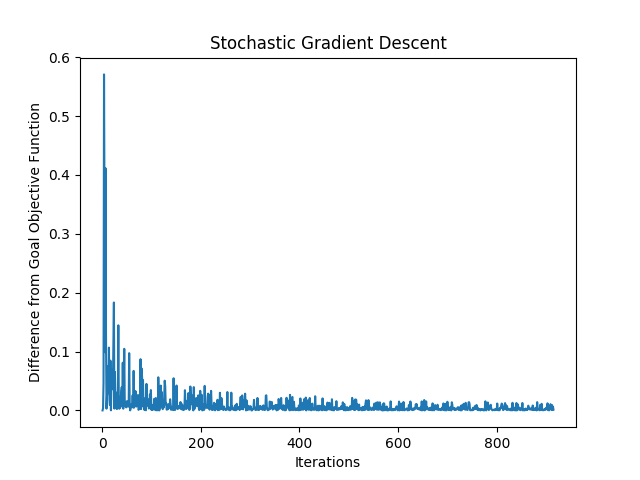
\includegraphics[width=\linewidth]{../P1/figs/plot_sgd.png}
        \end{subfigure}%
\caption*{It takes many more iterations for SGD to converge than batch descent. Furthermore, batch descent can converge on a more accurate answer (due to the randomness of SGD throwing things off). However, SGD runs much faster, even while taking more iterations. In practice, mini-batch SGD is often used as the best of both worlds.}
\end{figure}


\section{Linear Basis Function Regression}

\subsection{Closed-form Solution with Polynomial Basis}
% Replicate plots
Consider the basis function $$\Phi_M(x) = [\phi_0(x), \dots, \phi_M(x)],$$ where $\phi_k(x) = x^k$. Applying $\Phi_M$ to $\mathbf{X}$ gives the desired basis change, so we have the generalized linear model $$\mathbf Y = \Phi_M(\mathbf X) \cdot \bm \beta + \bm \epsilon,$$ which has the close-form solution $$\hat{\bm \beta} = (\Phi_M(\mathbf X)^T \Phi_M(\mathbf X))^{-1} \Phi_M(\mathbf X)^T \mathbf Y,$$
where $\hat{\bm \beta}$ is the maximum-likelihood estimator of the regression coefficients.

We ran regressions on the data using a few different degrees $(M = 0, 1, 3, 10)$.\footnotemark\ Below are plots of the resulting polynomial functions, compared to the given data and the true function:

\footnotetext{See the Appendix for the numerical values of the weights.}

\begin{figure}[H]
  \centering
  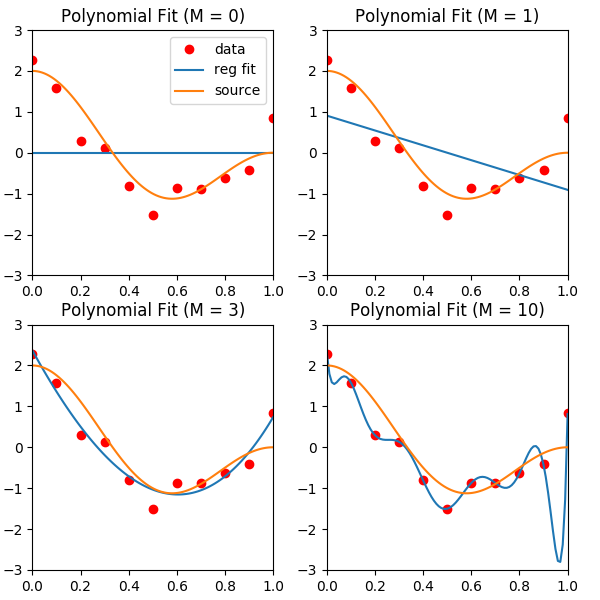
\includegraphics[width = 3.15in]{../P2/fig/part_1.png}
  \caption{M-Degree Polynomial Fit (M = 0, 1, 3, 10)}
\end{figure}

\subsection{Gradient Descent Solution with Polynomial Basis}
% Minimize SSE with Batch GD and SGD
% smallers thresholds produces slightly better fits when learn rate is small
% any threshold smaller than 1e-6 has similar results for learn rates we tested
% sgd is more sensitive to start point compared to bgd
% learn rate can't be too high or too low: doesn't converge when learn rate is too high, converges immediately when learn rate is too low (and when threshold is not adjusted accordingly)
% sgd is much more sensitive to learn rate as well
% stucks in local minima when degree is high -> more local minima


\subsection{Closed-form Solution with Cosine Function Basis}

\section{Ridge Regression}

\section{Sparsity and Lasso}

\section{Appendix}
% Coefficients in 2.1

\end{document}